\section{Score 1: no meaningful progress}
{\centering
\setlength{\tabcolsep}{1pt}\renewcommand{\arraystretch}{0.5}
\begin{tabular}{@{}cccccccc@{}}
{\scriptsize 1} & {\scriptsize 1} & {\scriptsize 1} & {\scriptsize 1} & {\scriptsize 1} & {\scriptsize 1} & {\scriptsize 1} & {\scriptsize 1} \\

\includegraphics[width=0.118\textwidth]{media/appendix/s1_window/f0.jpg} &

\includegraphics[width=0.118\textwidth]{media/appendix/s1_window/f1.jpg} &

\includegraphics[width=0.118\textwidth]{media/appendix/s1_window/f2.jpg} &

\includegraphics[width=0.118\textwidth]{media/appendix/s1_window/f3.jpg} &

\includegraphics[width=0.118\textwidth]{media/appendix/s1_window/f4.jpg} &

\includegraphics[width=0.118\textwidth]{media/appendix/s1_window/f5.jpg} &

\includegraphics[width=0.118\textwidth]{media/appendix/s1_window/f6.jpg} &

\includegraphics[width=0.118\textwidth]{media/appendix/s1_window/f7.jpg} \\
\end{tabular}\\[2pt]
{\footnotesize Window-close, random actions.}\par}
\vspace{8pt}
{\centering
\setlength{\tabcolsep}{1pt}\renewcommand{\arraystretch}{0.5}
\begin{tabular}{@{}cccccccc@{}}
{\scriptsize 1} & {\scriptsize 1} & {\scriptsize 1} & {\scriptsize 1} & {\scriptsize 1} & {\scriptsize 1} & {\scriptsize 1} & {\scriptsize 1} \\

\includegraphics[width=0.118\textwidth]{media/appendix/s1_door/f0.jpg} &

\includegraphics[width=0.118\textwidth]{media/appendix/s1_door/f1.jpg} &

\includegraphics[width=0.118\textwidth]{media/appendix/s1_door/f2.jpg} &

\includegraphics[width=0.118\textwidth]{media/appendix/s1_door/f3.jpg} &

\includegraphics[width=0.118\textwidth]{media/appendix/s1_door/f4.jpg} &

\includegraphics[width=0.118\textwidth]{media/appendix/s1_door/f5.jpg} &

\includegraphics[width=0.118\textwidth]{media/appendix/s1_door/f6.jpg} &

\includegraphics[width=0.118\textwidth]{media/appendix/s1_door/f7.jpg} \\
\end{tabular}\\[2pt]
{\footnotesize Door-open, wanders off, never reaches the door.}\par}
\vspace{8pt}
{\centering
\setlength{\tabcolsep}{1pt}\renewcommand{\arraystretch}{0.5}
\begin{tabular}{@{}cccccccc@{}}
{\scriptsize 1} & {\scriptsize 1} & {\scriptsize 1} & {\scriptsize 1} & {\scriptsize 1} & {\scriptsize 1} & {\scriptsize 1} & {\scriptsize 1} \\

\includegraphics[width=0.118\textwidth]{media/appendix/s1_push/f0.jpg} &

\includegraphics[width=0.118\textwidth]{media/appendix/s1_push/f1.jpg} &

\includegraphics[width=0.118\textwidth]{media/appendix/s1_push/f2.jpg} &

\includegraphics[width=0.118\textwidth]{media/appendix/s1_push/f3.jpg} &

\includegraphics[width=0.118\textwidth]{media/appendix/s1_push/f4.jpg} &

\includegraphics[width=0.118\textwidth]{media/appendix/s1_push/f5.jpg} &

\includegraphics[width=0.118\textwidth]{media/appendix/s1_push/f6.jpg} &

\includegraphics[width=0.118\textwidth]{media/appendix/s1_push/f7.jpg} \\
\end{tabular}\\[2pt]
{\footnotesize Push, moves the wrong way.}\par}
\vspace{8pt}
{\centering
\setlength{\tabcolsep}{1pt}\renewcommand{\arraystretch}{0.5}
\begin{tabular}{@{}cccccccc@{}}
{\scriptsize 1} & {\scriptsize 1} & {\scriptsize 1} & {\scriptsize 1} & {\scriptsize 1} & {\scriptsize 1} & {\scriptsize 1} & {\scriptsize 1} \\

\includegraphics[width=0.118\textwidth]{media/appendix/s1_hammer/f0.jpg} &

\includegraphics[width=0.118\textwidth]{media/appendix/s1_hammer/f1.jpg} &

\includegraphics[width=0.118\textwidth]{media/appendix/s1_hammer/f2.jpg} &

\includegraphics[width=0.118\textwidth]{media/appendix/s1_hammer/f3.jpg} &

\includegraphics[width=0.118\textwidth]{media/appendix/s1_hammer/f4.jpg} &

\includegraphics[width=0.118\textwidth]{media/appendix/s1_hammer/f5.jpg} &

\includegraphics[width=0.118\textwidth]{media/appendix/s1_hammer/f6.jpg} &

\includegraphics[width=0.118\textwidth]{media/appendix/s1_hammer/f7.jpg} \\
\end{tabular}\\[2pt]
{\footnotesize Hammer, random actions.}\par}
\vspace{8pt}

\bigskip

\section{Score 2: object approached but not engaged}
{\centering
\setlength{\tabcolsep}{1pt}\renewcommand{\arraystretch}{0.5}
\begin{tabular}{@{}cccccccc@{}}
{\scriptsize 2} & {\scriptsize 2} & {\scriptsize 2} & {\scriptsize 2} & {\scriptsize 2} & {\scriptsize 2} & {\scriptsize 2} & {\scriptsize 2} \\

\includegraphics[width=0.118\textwidth]{media/appendix/s2_faucet/f0.jpg} &

\includegraphics[width=0.118\textwidth]{media/appendix/s2_faucet/f1.jpg} &

\includegraphics[width=0.118\textwidth]{media/appendix/s2_faucet/f2.jpg} &

\includegraphics[width=0.118\textwidth]{media/appendix/s2_faucet/f3.jpg} &

\includegraphics[width=0.118\textwidth]{media/appendix/s2_faucet/f4.jpg} &

\includegraphics[width=0.118\textwidth]{media/appendix/s2_faucet/f5.jpg} &

\includegraphics[width=0.118\textwidth]{media/appendix/s2_faucet/f6.jpg} &

\includegraphics[width=0.118\textwidth]{media/appendix/s2_faucet/f7.jpg} \\
\end{tabular}\\[2pt]
{\footnotesize Faucet-open, reaches then freezes.}\par}
\vspace{8pt}
{\centering
\setlength{\tabcolsep}{1pt}\renewcommand{\arraystretch}{0.5}
\begin{tabular}{@{}cccccccc@{}}
{\scriptsize 1} & {\scriptsize 1} & {\scriptsize 1} & {\scriptsize 1} & {\scriptsize 2} & {\scriptsize 2} & {\scriptsize 2} & {\scriptsize 2} \\

\includegraphics[width=0.118\textwidth]{media/appendix/s2_door/f0.jpg} &

\includegraphics[width=0.118\textwidth]{media/appendix/s2_door/f1.jpg} &

\includegraphics[width=0.118\textwidth]{media/appendix/s2_door/f2.jpg} &

\includegraphics[width=0.118\textwidth]{media/appendix/s2_door/f3.jpg} &

\includegraphics[width=0.118\textwidth]{media/appendix/s2_door/f4.jpg} &

\includegraphics[width=0.118\textwidth]{media/appendix/s2_door/f5.jpg} &

\includegraphics[width=0.118\textwidth]{media/appendix/s2_door/f6.jpg} &

\includegraphics[width=0.118\textwidth]{media/appendix/s2_door/f7.jpg} \\
\end{tabular}\\[2pt]
{\footnotesize Door-open, reaches then freezes.}\par}
\vspace{8pt}
{\centering
\setlength{\tabcolsep}{1pt}\renewcommand{\arraystretch}{0.5}
\begin{tabular}{@{}cccccccc@{}}
{\scriptsize 1} & {\scriptsize 1} & {\scriptsize 1} & {\scriptsize 2} & {\scriptsize 2} & {\scriptsize 2} & {\scriptsize 2} & {\scriptsize 2} \\

\includegraphics[width=0.118\textwidth]{media/appendix/s2_sweep/f0.jpg} &

\includegraphics[width=0.118\textwidth]{media/appendix/s2_sweep/f1.jpg} &

\includegraphics[width=0.118\textwidth]{media/appendix/s2_sweep/f2.jpg} &

\includegraphics[width=0.118\textwidth]{media/appendix/s2_sweep/f3.jpg} &

\includegraphics[width=0.118\textwidth]{media/appendix/s2_sweep/f4.jpg} &

\includegraphics[width=0.118\textwidth]{media/appendix/s2_sweep/f5.jpg} &

\includegraphics[width=0.118\textwidth]{media/appendix/s2_sweep/f6.jpg} &

\includegraphics[width=0.118\textwidth]{media/appendix/s2_sweep/f7.jpg} \\
\end{tabular}\\[2pt]
{\footnotesize Sweep-into, touches then freezes.}\par}
\vspace{8pt}
{\centering
\setlength{\tabcolsep}{1pt}\renewcommand{\arraystretch}{0.5}
\begin{tabular}{@{}cccccccc@{}}
{\scriptsize 1} & {\scriptsize 1} & {\scriptsize 1} & {\scriptsize 1} & {\scriptsize 2} & {\scriptsize 2} & {\scriptsize 2} & {\scriptsize 2} \\

\includegraphics[width=0.118\textwidth]{media/appendix/s2_drawer/f0.jpg} &

\includegraphics[width=0.118\textwidth]{media/appendix/s2_drawer/f1.jpg} &

\includegraphics[width=0.118\textwidth]{media/appendix/s2_drawer/f2.jpg} &

\includegraphics[width=0.118\textwidth]{media/appendix/s2_drawer/f3.jpg} &

\includegraphics[width=0.118\textwidth]{media/appendix/s2_drawer/f4.jpg} &

\includegraphics[width=0.118\textwidth]{media/appendix/s2_drawer/f5.jpg} &

\includegraphics[width=0.118\textwidth]{media/appendix/s2_drawer/f6.jpg} &

\includegraphics[width=0.118\textwidth]{media/appendix/s2_drawer/f7.jpg} \\
\end{tabular}\\[2pt]
{\footnotesize Drawer-open, reaches the handle but never grips it.}\par}
\vspace{8pt}

\bigskip

\section{Score 3: object engaged, partial progress}
{\centering
\setlength{\tabcolsep}{1pt}\renewcommand{\arraystretch}{0.5}
\begin{tabular}{@{}cccccccc@{}}
{\scriptsize 1} & {\scriptsize 2} & {\scriptsize 2} & {\scriptsize 2} & {\scriptsize 3} & {\scriptsize 3} & {\scriptsize 3} & {\scriptsize 3} \\

\includegraphics[width=0.118\textwidth]{media/appendix/s3_bball/f0.jpg} &

\includegraphics[width=0.118\textwidth]{media/appendix/s3_bball/f1.jpg} &

\includegraphics[width=0.118\textwidth]{media/appendix/s3_bball/f2.jpg} &

\includegraphics[width=0.118\textwidth]{media/appendix/s3_bball/f3.jpg} &

\includegraphics[width=0.118\textwidth]{media/appendix/s3_bball/f4.jpg} &

\includegraphics[width=0.118\textwidth]{media/appendix/s3_bball/f5.jpg} &

\includegraphics[width=0.118\textwidth]{media/appendix/s3_bball/f6.jpg} &

\includegraphics[width=0.118\textwidth]{media/appendix/s3_bball/f7.jpg} \\
\end{tabular}\\[2pt]
{\footnotesize Basketball, grasps the ball but never lifts it to the hoop.}\par}
\vspace{8pt}
{\centering
\setlength{\tabcolsep}{1pt}\renewcommand{\arraystretch}{0.5}
\begin{tabular}{@{}cccccccc@{}}
{\scriptsize 1} & {\scriptsize 1} & {\scriptsize 1} & {\scriptsize 2} & {\scriptsize 3} & {\scriptsize 3} & {\scriptsize 3} & {\scriptsize 3} \\

\includegraphics[width=0.118\textwidth]{media/appendix/s3_pickpl/f0.jpg} &

\includegraphics[width=0.118\textwidth]{media/appendix/s3_pickpl/f1.jpg} &

\includegraphics[width=0.118\textwidth]{media/appendix/s3_pickpl/f2.jpg} &

\includegraphics[width=0.118\textwidth]{media/appendix/s3_pickpl/f3.jpg} &

\includegraphics[width=0.118\textwidth]{media/appendix/s3_pickpl/f4.jpg} &

\includegraphics[width=0.118\textwidth]{media/appendix/s3_pickpl/f5.jpg} &

\includegraphics[width=0.118\textwidth]{media/appendix/s3_pickpl/f6.jpg} &

\includegraphics[width=0.118\textwidth]{media/appendix/s3_pickpl/f7.jpg} \\
\end{tabular}\\[2pt]
{\footnotesize Pick-place, picks up the puck then drops it.}\par}
\vspace{8pt}
{\centering
\setlength{\tabcolsep}{1pt}\renewcommand{\arraystretch}{0.5}
\begin{tabular}{@{}cccccccc@{}}
{\scriptsize 1} & {\scriptsize 1} & {\scriptsize 1} & {\scriptsize 2} & {\scriptsize 3} & {\scriptsize 3} & {\scriptsize 3} & {\scriptsize 3} \\

\includegraphics[width=0.118\textwidth]{media/appendix/s3_push/f0.jpg} &

\includegraphics[width=0.118\textwidth]{media/appendix/s3_push/f1.jpg} &

\includegraphics[width=0.118\textwidth]{media/appendix/s3_push/f2.jpg} &

\includegraphics[width=0.118\textwidth]{media/appendix/s3_push/f3.jpg} &

\includegraphics[width=0.118\textwidth]{media/appendix/s3_push/f4.jpg} &

\includegraphics[width=0.118\textwidth]{media/appendix/s3_push/f5.jpg} &

\includegraphics[width=0.118\textwidth]{media/appendix/s3_push/f6.jpg} &

\includegraphics[width=0.118\textwidth]{media/appendix/s3_push/f7.jpg} \\
\end{tabular}\\[2pt]
{\footnotesize Push the puck to the goal, then slides it sideways instead.}\par}
\vspace{8pt}
{\centering
\setlength{\tabcolsep}{1pt}\renewcommand{\arraystretch}{0.5}
\begin{tabular}{@{}cccccccc@{}}
{\scriptsize 1} & {\scriptsize 1} & {\scriptsize 1} & {\scriptsize 2} & {\scriptsize 3} & {\scriptsize 3} & {\scriptsize 2} & {\scriptsize 2} \\

\includegraphics[width=0.118\textwidth]{media/appendix/s3_coffee/f0.jpg} &

\includegraphics[width=0.118\textwidth]{media/appendix/s3_coffee/f1.jpg} &

\includegraphics[width=0.118\textwidth]{media/appendix/s3_coffee/f2.jpg} &

\includegraphics[width=0.118\textwidth]{media/appendix/s3_coffee/f3.jpg} &

\includegraphics[width=0.118\textwidth]{media/appendix/s3_coffee/f4.jpg} &

\includegraphics[width=0.118\textwidth]{media/appendix/s3_coffee/f5.jpg} &

\includegraphics[width=0.118\textwidth]{media/appendix/s3_coffee/f6.jpg} &

\includegraphics[width=0.118\textwidth]{media/appendix/s3_coffee/f7.jpg} \\
\end{tabular}\\[2pt]
{\footnotesize Coffee-push, pushes partway then lifts away.}\par}
\vspace{8pt}

\bigskip

\section{Score 4: near-complete but ultimately fails}
{\centering
\setlength{\tabcolsep}{1pt}\renewcommand{\arraystretch}{0.5}
\begin{tabular}{@{}cccccccc@{}}
{\scriptsize 1} & {\scriptsize 1} & {\scriptsize 2} & {\scriptsize 3} & {\scriptsize 4} & {\scriptsize 3} & {\scriptsize 3} & {\scriptsize 3} \\

\includegraphics[width=0.118\textwidth]{media/appendix/s4_pickpl/f0.jpg} &

\includegraphics[width=0.118\textwidth]{media/appendix/s4_pickpl/f1.jpg} &

\includegraphics[width=0.118\textwidth]{media/appendix/s4_pickpl/f2.jpg} &

\includegraphics[width=0.118\textwidth]{media/appendix/s4_pickpl/f3.jpg} &

\includegraphics[width=0.118\textwidth]{media/appendix/s4_pickpl/f4.jpg} &

\includegraphics[width=0.118\textwidth]{media/appendix/s4_pickpl/f5.jpg} &

\includegraphics[width=0.118\textwidth]{media/appendix/s4_pickpl/f6.jpg} &

\includegraphics[width=0.118\textwidth]{media/appendix/s4_pickpl/f7.jpg} \\
\end{tabular}\\[2pt]
{\footnotesize Pick-place, grasps the puck and carries it close to the goal but ultimately drops it.}\par}
\vspace{8pt}
{\centering
\setlength{\tabcolsep}{1pt}\renewcommand{\arraystretch}{0.5}
\begin{tabular}{@{}cccccccc@{}}
{\scriptsize 3} & {\scriptsize 3} & {\scriptsize 3} & {\scriptsize 3} & {\scriptsize 4} & {\scriptsize 4} & {\scriptsize 4} & {\scriptsize 4} \\

\includegraphics[width=0.118\textwidth]{media/appendix/s4_boxcl/f0.jpg} &

\includegraphics[width=0.118\textwidth]{media/appendix/s4_boxcl/f1.jpg} &

\includegraphics[width=0.118\textwidth]{media/appendix/s4_boxcl/f2.jpg} &

\includegraphics[width=0.118\textwidth]{media/appendix/s4_boxcl/f3.jpg} &

\includegraphics[width=0.118\textwidth]{media/appendix/s4_boxcl/f4.jpg} &

\includegraphics[width=0.118\textwidth]{media/appendix/s4_boxcl/f5.jpg} &

\includegraphics[width=0.118\textwidth]{media/appendix/s4_boxcl/f6.jpg} &

\includegraphics[width=0.118\textwidth]{media/appendix/s4_boxcl/f7.jpg} \\
\end{tabular}\\[2pt]
{\footnotesize Box-close, nearly closes then misplaces.}\par}
\vspace{8pt}
{\centering
\setlength{\tabcolsep}{1pt}\renewcommand{\arraystretch}{0.5}
\begin{tabular}{@{}cccccccc@{}}
{\scriptsize 1} & {\scriptsize 2} & {\scriptsize 2} & {\scriptsize 3} & {\scriptsize 4} & {\scriptsize 4} & {\scriptsize 4} & {\scriptsize 4} \\

\includegraphics[width=0.118\textwidth]{media/appendix/s4_plate/f0.jpg} &

\includegraphics[width=0.118\textwidth]{media/appendix/s4_plate/f1.jpg} &

\includegraphics[width=0.118\textwidth]{media/appendix/s4_plate/f2.jpg} &

\includegraphics[width=0.118\textwidth]{media/appendix/s4_plate/f3.jpg} &

\includegraphics[width=0.118\textwidth]{media/appendix/s4_plate/f4.jpg} &

\includegraphics[width=0.118\textwidth]{media/appendix/s4_plate/f5.jpg} &

\includegraphics[width=0.118\textwidth]{media/appendix/s4_plate/f6.jpg} &

\includegraphics[width=0.118\textwidth]{media/appendix/s4_plate/f7.jpg} \\
\end{tabular}\\[2pt]
{\footnotesize Plate-slide, almost there then off-line.}\par}
\vspace{8pt}
{\centering
\setlength{\tabcolsep}{1pt}\renewcommand{\arraystretch}{0.5}
\begin{tabular}{@{}cccccccc@{}}
{\scriptsize 1} & {\scriptsize 1} & {\scriptsize 1} & {\scriptsize 2} & {\scriptsize 4} & {\scriptsize 4} & {\scriptsize 4} & {\scriptsize 4} \\

\includegraphics[width=0.118\textwidth]{media/appendix/s4_button/f0.jpg} &

\includegraphics[width=0.118\textwidth]{media/appendix/s4_button/f1.jpg} &

\includegraphics[width=0.118\textwidth]{media/appendix/s4_button/f2.jpg} &

\includegraphics[width=0.118\textwidth]{media/appendix/s4_button/f3.jpg} &

\includegraphics[width=0.118\textwidth]{media/appendix/s4_button/f4.jpg} &

\includegraphics[width=0.118\textwidth]{media/appendix/s4_button/f5.jpg} &

\includegraphics[width=0.118\textwidth]{media/appendix/s4_button/f6.jpg} &

\includegraphics[width=0.118\textwidth]{media/appendix/s4_button/f7.jpg} \\
\end{tabular}\\[2pt]
{\footnotesize Button-press, almost presses then stops.}\par}
\vspace{8pt}

\bigskip

\section{FailSafe (ManiSkill)}
{\centering
\setlength{\tabcolsep}{1pt}\renewcommand{\arraystretch}{0.5}
\begin{tabular}{@{}cccccccc@{}}
{\scriptsize 1} & {\scriptsize 1} & {\scriptsize 2} & {\scriptsize 4} & {\scriptsize 4} & {\scriptsize 4} & {\scriptsize 1} & {\scriptsize 1} \\
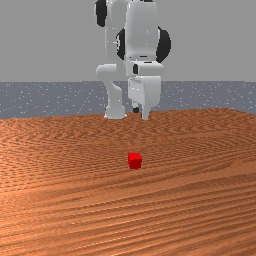
\includegraphics[width=0.118\textwidth]{media/appendix/fs_pick/f0.jpg} &
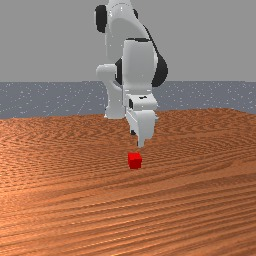
\includegraphics[width=0.118\textwidth]{media/appendix/fs_pick/f1.jpg} &
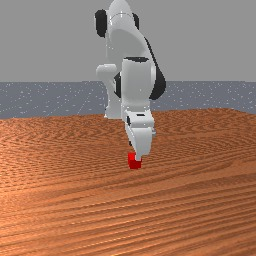
\includegraphics[width=0.118\textwidth]{media/appendix/fs_pick/f2.jpg} &
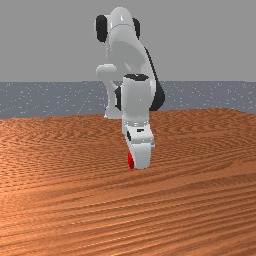
\includegraphics[width=0.118\textwidth]{media/appendix/fs_pick/f3.jpg} &
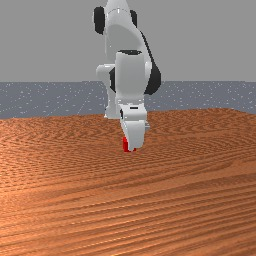
\includegraphics[width=0.118\textwidth]{media/appendix/fs_pick/f4.jpg} &
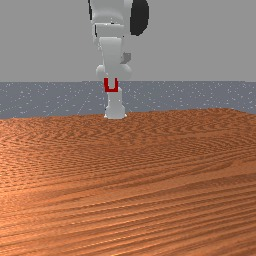
\includegraphics[width=0.118\textwidth]{media/appendix/fs_pick/f5.jpg} &
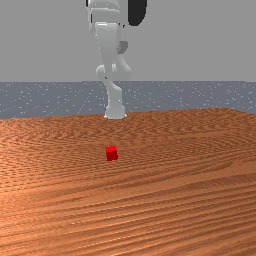
\includegraphics[width=0.118\textwidth]{media/appendix/fs_pick/f6.jpg} &
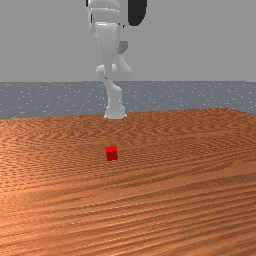
\includegraphics[width=0.118\textwidth]{media/appendix/fs_pick/f7.jpg} \\
\end{tabular}\\[2pt]
{\footnotesize Pick, grasps and lifts then releases.}\par}
\vspace{8pt}
{\centering
\setlength{\tabcolsep}{1pt}\renewcommand{\arraystretch}{0.5}
\begin{tabular}{@{}cccccccc@{}}
{\scriptsize 1} & {\scriptsize 1} & {\scriptsize 1} & {\scriptsize 2} & {\scriptsize 2} & {\scriptsize 2} & {\scriptsize 2} & {\scriptsize 4} \\

\includegraphics[width=0.118\textwidth]{media/appendix/fs_push/f0.jpg} &

\includegraphics[width=0.118\textwidth]{media/appendix/fs_push/f1.jpg} &

\includegraphics[width=0.118\textwidth]{media/appendix/fs_push/f2.jpg} &

\includegraphics[width=0.118\textwidth]{media/appendix/fs_push/f3.jpg} &

\includegraphics[width=0.118\textwidth]{media/appendix/fs_push/f4.jpg} &

\includegraphics[width=0.118\textwidth]{media/appendix/fs_push/f5.jpg} &

\includegraphics[width=0.118\textwidth]{media/appendix/fs_push/f6.jpg} &

\includegraphics[width=0.118\textwidth]{media/appendix/fs_push/f7.jpg} \\
\end{tabular}\\[2pt]
{\footnotesize Push, pushes toward the goal then stalls.}\par}
\vspace{8pt}
{\centering
\setlength{\tabcolsep}{1pt}\renewcommand{\arraystretch}{0.5}
\begin{tabular}{@{}cccccccc@{}}
{\scriptsize 1} & {\scriptsize 1} & {\scriptsize 2} & {\scriptsize 2} & {\scriptsize 3} & {\scriptsize 3} & {\scriptsize 1} & {\scriptsize 1} \\

\includegraphics[width=0.118\textwidth]{media/appendix/fs_stack/f0.jpg} &

\includegraphics[width=0.118\textwidth]{media/appendix/fs_stack/f1.jpg} &

\includegraphics[width=0.118\textwidth]{media/appendix/fs_stack/f2.jpg} &

\includegraphics[width=0.118\textwidth]{media/appendix/fs_stack/f3.jpg} &

\includegraphics[width=0.118\textwidth]{media/appendix/fs_stack/f4.jpg} &

\includegraphics[width=0.118\textwidth]{media/appendix/fs_stack/f5.jpg} &

\includegraphics[width=0.118\textwidth]{media/appendix/fs_stack/f6.jpg} &

\includegraphics[width=0.118\textwidth]{media/appendix/fs_stack/f7.jpg} \\
\end{tabular}\\[2pt]
{\footnotesize Stack, carries the cube then drops it.}\par}
\vspace{8pt}
